\afuncT{clip}{Clip. Computes the generalized double clip of two views. See \cvl{} specification for more information.}{selectionOperations}
\\\cvsiplh
\afh
{
\ttfamily
\\\hspace*{.04\textwidth}\begin{tabular}[H]{l}
void vsip\_mclip\_d(\\*\hspace*{1cm}const vsip\_mview\_d*, vsip\_scalar\_d, vsip\_scalar\_d,\\*\hspace*{1cm}vsip\_scalar\_d, vsip\_scalar\_d, const vsip\_mview\_d*);\\
void vsip\_mclip\_f(\\*\hspace*{1cm}const vsip\_mview\_f*, vsip\_scalar\_f, vsip\_scalar\_f,\\*\hspace*{1cm}vsip\_scalar\_f, vsip\_scalar\_f, const vsip\_mview\_f*);\\
void vsip\_mclip\_i(\\*\hspace*{1cm}const vsip\_mview\_i*, vsip\_scalar\_i, vsip\_scalar\_i,\\*\hspace*{1cm}vsip\_scalar\_i, vsip\_scalar\_i, const vsip\_mview\_i*);\\
void vsip\_mclip\_si(\\*\hspace*{1cm}const vsip\_mview\_si*, vsip\_scalar\_si, vsip\_scalar\_si,\\*\hspace*{1cm}vsip\_scalar\_si, vsip\_scalar\_si, const vsip\_mview\_si*);\\
void vsip\_vclip\_d(\\*\hspace*{1cm}const vsip\_vview\_d*, vsip\_scalar\_d, vsip\_scalar\_d,\\*\hspace*{1cm}vsip\_scalar\_d, vsip\_scalar\_d, const vsip\_vview\_d*);\\
void vsip\_vclip\_f(\\*\hspace*{1cm}const vsip\_vview\_f*, vsip\_scalar\_f, vsip\_scalar\_f,\\*\hspace*{1cm}vsip\_scalar\_f, vsip\_scalar\_f, const vsip\_vview\_f*);\\
void vsip\_vclip\_i(\\*\hspace*{1cm}const vsip\_vview\_i*, vsip\_scalar\_i, vsip\_scalar\_i,\\*\hspace*{1cm}vsip\_scalar\_i, vsip\_scalar\_i, const vsip\_vview\_i*);\\
void vsip\_vclip\_si(\\*\hspace*{1cm}const vsip\_vview\_si*, vsip\_scalar\_si, vsip\_scalar\_si,\\*\hspace*{1cm}vsip\_scalar\_si, vsip\_scalar\_si, const vsip\_vview\_si*);\\
void vsip\_vclip\_uc(\\*\hspace*{1cm}const vsip\_vview\_uc*, vsip\_scalar\_uc, vsip\_scalar\_uc,\\*\hspace*{1cm}vsip\_scalar\_uc, vsip\_scalar\_uc, const vsip\_vview\_uc*);\\
\end{tabular}
}
\\\pyjvsiph
\viewmthd{No}{NA}{NA}{NA}
\apyfunc{Yes}{\ttbf{clip(in,t1,t2,c1,c2,out)}}
\inputminted[linenos=true,resetmargins=true,xleftmargin=.12\textwidth,fontfamily=tt,fontsize=\small]{python}{./pyJvsip_examples/eXclip.py}
\hspace*{.08\textwidth}{\rmfamily For result see figure \ref{fig:ClipExample}.}
\begin{figure}[t]\centering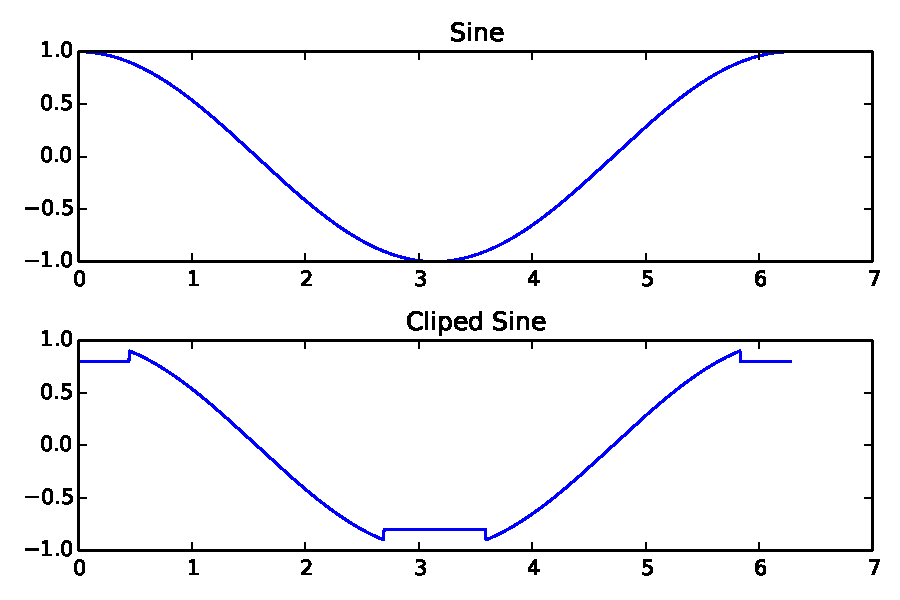
\includegraphics[width=0.8\textwidth]{eXclip}\caption{Clip Example}\label{fig:ClipExample}\end{figure}
\pyComment{
\item{The clip function works much the same as \cvl{} except the output is returned. In line 6 of the example we used the \ttbf{empty} method to create the output vector and saved a reference in the left value.}
\item{The \ttbf{clip} function is a bit complicated. See the \cvl{} specification for more complete details.}
\item{The \ttbf{view} \ttbf{in} is clipped according to the rules of the function. The clipping checks are set by \ttbf{t1} and \ttbf{t2} and the clip values are set by \ttbf{c1} and \ttbf{c2} accordingly. The output is placed in \ttbf{out}. If \ttbf{in==out} then the function is done in-place}
}